\section{Fundamental Concepts, Theories, and Background}

This chapter covers aspects related to all the fundamental concepts and theories that support understanding of the research problem, as well as the procedures carried out. Additionally, it is necessary to incorporate works by other authors related to the research topic that may serve as references.

According to Grinnell, Williams, and Unrau\cite{grinnell2009}, the literature review in a proposal or protocol fulfills five basic functions:

\begin{enumerate}[label=\alph*)]
	
	\item Ensure that reviewers or evaluators fully understand the issues or topics related to the research problem. Dahlberg, Wittink, and Gallo\cite{dahlberg2010} point out a common mistake that often appears in proposals: assuming that readers are familiar with the importance of the problem. Therefore, to avoid this error, we must explicitly state its relevance, significance, and necessity.

	\item Indicate the differences and similarities between the current study and previous ones (differentiation).

	\item Position the research within the current body of knowledge in a given field (in this sense, the literature review or background should show how the study fits into an area of knowledge or professional practice).

	\item Describe how the results will contribute to the field of knowledge or practice in which the project is embedded (what questions it will answer, what controversies it will help clarify, how it will advance knowledge or technology, etc.).

	\item Introduce and conceptualize the variables that will be considered in the study (and ideally show potential relationships between the variables).

\end{enumerate}

For their part, Stanford University\cite{stanford2017} and Betkerur\cite{betkerur2008} state that the literature review allows readers to become familiar with the problem under study, describes the work conducted by some colleagues both locally and internationally around the problem statement and similar issues, and helps you as a researcher to understand the difficulties those colleagues faced so you can anticipate them.

\begin{figure}[ht]
	\centering
	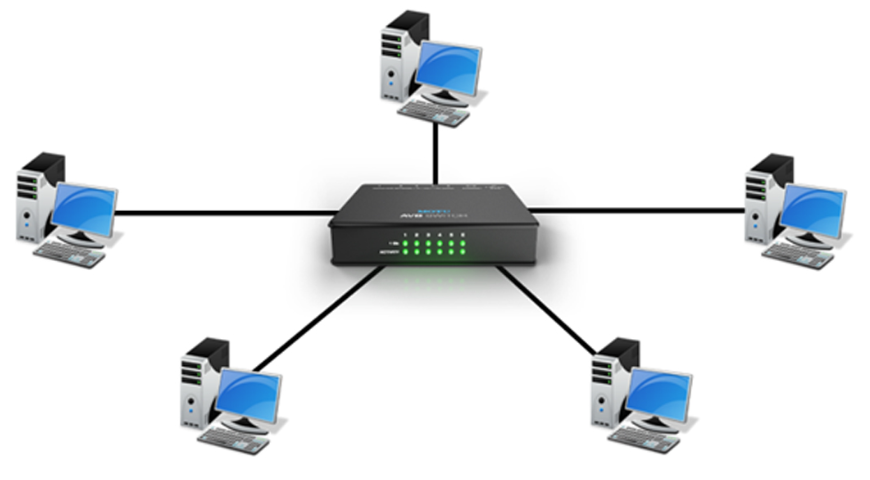
\includegraphics[width=0.5\textwidth]{img/hub.png}
	\caption{This is a sample image.}
\end{figure}

All theories, concepts, descriptions, ideas, and background information included in this section must be properly cited and referenced. The citation style used throughout the paper will be IEEE\footnote{IEEE uses a numerical citation system. The sources are indicated by a number in square brackets within the text, which corresponds to the full reference that must be included in the final bibliography. For more information on this system, consult \url{https://journals.ieeeauthorcenter.ieee.org/wp-content/uploads/sites/7/IEEE_Reference_Guide.pdf}}.

\subsection{Fundamental Concepts}
This section may include all concepts, definitions, and descriptions necessary to delve into the researched topic and help understand the problem being addressed.

\subsection{Background}
Previous studies and experiences related to the researched topic and a summary of the most important findings that help visualize the current state of science in the area of the addressed problem. The theoretical exposition should flow from the oldest to the most recent and from the broadest to the specific subject of the work.

At least five background studies will be required. The incorporated background must help to understand the current state of the topic and also provide a general overview of the solutions proposed by other authors to problems directly or indirectly related to the problem addressed in this work.

A proper literature review (focused on the problem statement and hypothesis, with current and relevant references) is a good indicator that, as a researcher, you have mastered the existing state of knowledge on your topic. The literature review is not a list of references, nor summaries of them, nor a compilation of vaguely related sources. Instead, it represents an integration of selectively chosen references that fulfill the outlined functions. In a few pages, you should discuss what studies have been previously conducted on the problem you will investigate and their main findings. When writing this section, you need to be very direct and concise, avoiding long definitions of concepts. We stress this: only include previous research that has specifically addressed your problem of interest. For instance, Trupke and Strassnig\cite{trupke2017} suggest including around 10 significant references. Including too many primary sources (especially when not directly linked to the topic) can bore the reader and leave out important references, which also suggests a lack of knowledge about a problem or phenomenon.

Finally, the links between questions and objectives, the theory, and the selected methods must be clear. Although this section does not present the entire methodology, you should include one or two paragraphs that connect theory with method at the end of the background section. This also helps to bridge this section with the next.

Some examples of initial wording for background paragraphs are shown in the following box:

\vspace{0.5cm}

\begin{table}[h]
	\begin{tabular}{| m{12cm} |}
		\hline
		\vspace{0.5cm}
		“In the literature relevant (linked, related, prior...) to our problem statement, it has been found that... (references) and... (reference)”

		\vspace{0.5cm}

		“Previous studies (references) have concluded that…”

		\vspace{0.5cm}

		“The background shows us that... (references)”

		\vspace{0.5cm}

		“Research has made it clear that... (references)...”

		\vspace{0.5cm}

		“On the other hand, it has also been discovered (demonstrated, highlighted, indicated... (references)...)”

		\vspace{0.5cm}

		“Furthermore, it has been concluded that... (references)”

		\vspace{0.5cm}

		\\
		\hline
	\end{tabular}
\end{table}

Also here is a example of a code, this can be changed and can be updated:
\noindent\textbf{Code example}
\begin{lstlisting}
// 1 Hz square wave on RC2
void init_compare(void){
    TRISC2_bit = 0;
    CCP1CON = 0b00000010;     // Compare, toggle output
    CCPTMRS0.C1TSEL = 0;      // Timer1
    CCPR1H = 0xF4;            
    CCPR1L = 0x24;
    T1CON = 0b00110001;       // Timer1 at 1 MHz tick
}
\end{lstlisting}